\documentclass[tikz,border=2pt]{standalone}
\usepackage{tikz}
\usetikzlibrary{positioning, arrows.meta, calc}
\usepackage{xcolor}

\definecolor{research}{HTML}{0077BB}
\definecolor{policy}{HTML}{EE7733}
\definecolor{sharedbg}{HTML}{444444}

\tikzset{
  base/.style={draw, rounded corners=3pt, align=center,
               inner xsep=6pt, inner ysep=5pt, line width=0.5pt},
  dimbox/.style={base, fill=sharedbg!6, draw=sharedbg, text width=4.8cm, minimum height=1.2cm},
  levelbox/.style={base, fill=white, draw=gray!60, text width=4.8cm, minimum height=0.8cm, font=\footnotesize},
  arrow/.style={-{Stealth[length=2mm]}, draw=gray!70, line width=0.5pt},
  label/.style={font=\footnotesize\bfseries, align=center, text=black},
}

\begin{document}
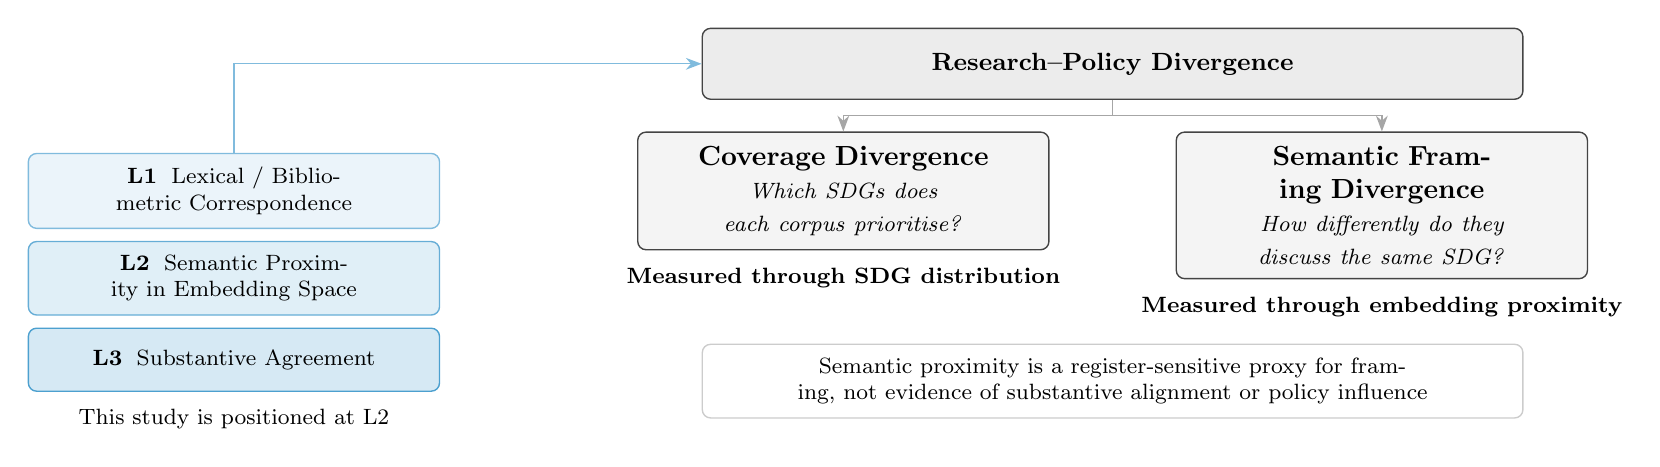
\begin{tikzpicture}[node distance=0.5cm and 0.3cm]

%% ====================  TOP TITLE  ====================

\node[base, fill=sharedbg!10, draw=sharedbg, text width=10cm,
      minimum height=0.9cm, font=\bfseries\small]
  (top) {Research--Policy Divergence};

%% ====================  TWO COLUMNS  ====================

\node[dimbox, below left=0.4cm and 0.8cm of top.south]
  (cov) {\textbf{Coverage Divergence}\\ \footnotesize \textit{Which SDGs does each corpus prioritise?}};

\node[dimbox, below right=0.4cm and 0.8cm of top.south]
  (sem) {\textbf{Semantic Framing Divergence}\\ \footnotesize \textit{How differently do they discuss the same SDG?}};

\node[label, below=0.1cm of cov]
  (cov_label) {Measured through SDG distribution};

\node[label, below=0.1cm of sem]
  (sem_label) {Measured through embedding proximity};

%% ====================  THREE-LEVEL LADDER  ====================

\node[levelbox, fill=research!8, draw=research!50, left=2.5cm of cov]
  (l1) {\textbf{L1}\; Lexical / Bibliometric Correspondence};
\node[levelbox, fill=research!12, draw=research!60, below=0.15cm of l1]
  (l2) {\textbf{L2}\; Semantic Proximity in Embedding Space};
\node[levelbox, fill=research!16, draw=research!70, below=0.15cm of l2]
  (l3) {\textbf{L3}\; Substantive Agreement};

\node[label, below=0.1cm of l3, text width=4.5cm, font=\footnotesize]
  (ladder_label) {This study is positioned at L2};

%% connecting ladder to title
\draw[arrow, draw=research!50] (l1.north) |- (top.west);

%% ====================  ARROWS  ====================

\draw[arrow] (top.south) -- ++(0,-0.2cm) -| (cov.north);
\draw[arrow] (top.south) -- ++(0,-0.2cm) -| (sem.north);

%% ====================  BOTTOM NOTE  ====================

\node[base, fill=white, draw=gray!40, text width=10cm,
      minimum height=0.7cm, font=\footnotesize,
      below=1.0cm of $(cov.south)!0.5!(sem.south)$]
  (note) {Semantic proximity is a register-sensitive proxy for framing, not evidence of substantive alignment or policy influence};

\end{tikzpicture}
\end{document}
